\documentclass[sigconf]{acmart}
% defining the \BibTeX command - from Oren Patashnik's original BibTeX documentation.
\def\BibTeX{{\rm B\kern-.05em{\sc i\kern-.025em b}\kern-.08emT\kern-.1667em\lower.7ex\hbox{E}\kern-.125emX}}
% Remove the annoying stuff
\settopmatter{printacmref=false} % Removes citation information below abstract
\renewcommand\footnotetextcopyrightpermission[1]{} % removes footnote with conference information in first column
\pagestyle{plain} % removes running headers

\usepackage{Nikolai}

\usepackage{lipsum}





\begin{document}

%
% The "title" command has an optional parameter, allowing the author to define a "short title" to be used in page headers.
\title{CMIS Hand-in 2: Finite Difference Methods 2}

\author{Nikolai Plambech Nielsen}
\email{lpk331@alumni.ku.dk}
\affiliation{%
  \institution{Niels Bohr Institute, University of Copenhagen}
}


\maketitle

\section{Introduction}


\section{Semi-Lagrangian implicit time integration: solving the advection equation}
In this problem we encounter the advection equation:
\begin{equation}\label{key}
	\frac{D \phi}{D t} = (\V{u} \D \grad) \phi + \diff{\phi}{t}
\end{equation}
Where $ D\phi/Dt $ is the particle derivative of the scalar field $ \phi $, and $ \V{u} $ is the associated velocity field. We set $ D\phi/Dt = 0 $ such that no dissipation occurs for the system:
\begin{equation}\label{key}
	 \diff{\phi}{t} = -(\V{u} \D \grad) \phi
\end{equation} 
The advection equation describes the flow of some scalar field $ \phi $ in a velocity field $ \V{u} $. This could for example describe the motion of food colouring in a pool of water. Then $ \phi $ would be the density of the food colouring molecules, whilst $ \V{u} $ would be the flow of the water in the pool.

The idea behind semi-lagrangian time integration is to use this property of the advection equation, and directly use the values of the scalar field at the previous times step. Specifically we treat our grid points as particles floating along the vector field. At a previous time, the grid point particles (to first order) were at
\begin{equation}\label{key}
	\V{x}^{t - \Delta t} = \V{x}^t - \Delta t \V{u}
\end{equation}
we then use the the value of the field at these points as the value for $ phi $ on the grid points, for the next time step:
\begin{equation}\label{key}
	\phi(\V{x}^{t}) \leftarrow \phi(\V{x}^t - \Delta t \V{u}) 
\end{equation}
The problem then, is that we are not guaranteed, that the grid point particles hit a grid point position, and as such we might not know the value of $ \phi(\V{x}^t - \Delta t \V{u}) $. To get around this we use a bilinear interpolation between the four nearest grid points to $ \V{x}^{t - \Delta t} $, and use this interpolated value as the true value.

For this problem we use a velocity field of $ \V{u} = (y, -x)^T $, corresponding to constant circular motion in the clockwise direction. For the scalar field we use a sum of Gaussian functions. If we choose the width of the Gaussians to be sufficiently small, and a large domain, virtually all the points of $ \phi $ that are non-zero will be nowhere near the boundary of the domain. This ensures that a bilinear interpolation always has enough points to use for the interpolation.

With this vector field, we expect the scalar field to rotate in time, with a period of $ 2\pi $. We can then perform an (approximate) full rotation in $ N $ steps by defining $ \Delta t = 2\pi/N $. It is only approximate due to the truncation error present when discretising the system.


\subsection{Experiments}
\begin{figure}
	\centering
	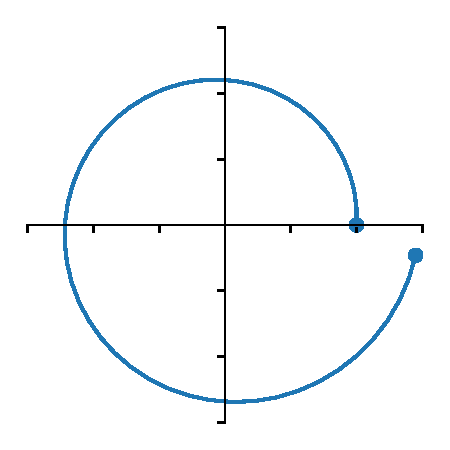
\includegraphics[width=0.7\linewidth]{spiral.pdf}
	\caption{Typical trajectory of a grid point after $ N $ iterations of semi-Lagrangian time integration (if the grid point was continually interpreted as a particle).}
	\label{fig:spiral}
\end{figure}
For this problem I perform two experiments. In the first I want to test how the rotation depends on the time step, and in the second I test how much bleeding occurs, again as a function of the time step and grid spacing.

\begin{figure}
	\centering
	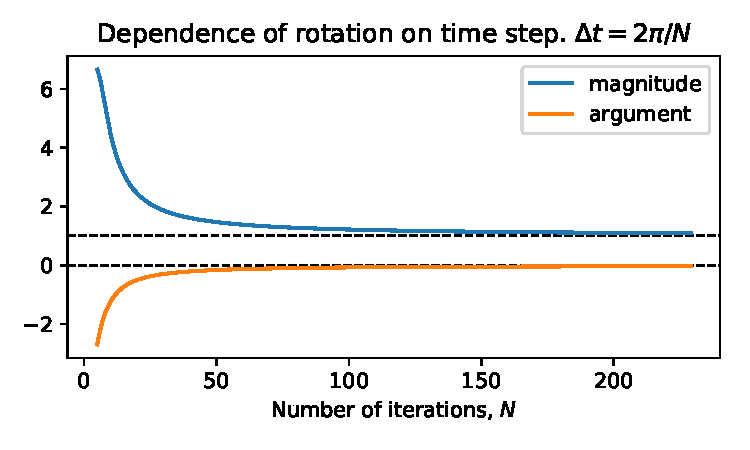
\includegraphics[width=\linewidth]{rotation_dependence.pdf}
	\caption{Argument and ratio of magnitudes calculated as a function of the time step size $  \Delta t $. As $ \Delta t $ decreases, the system approaches a full revolution, corresponding to an argument of 0 and a magnitude ratio of 1.}
	\label{fig:rotation}
\end{figure}

To test the rotation, I take a point, say $ \V{x} = (2,0)^T $ and backtrace $ N $ times to get $ \V{x}' $, corresponding to one rotation of the whole grid, and compare the magnitude and argument of $ \V{x}' $ to that of $ \V{x} $. An example of the trajectory is seen in figure \ref{fig:spiral}, with $ \Delta t = \pi/25\approx 0.126 $. In figure \ref{fig:rotation} the ratio of magnitudes $ ||\V{x}'|| / ||\V{x}|| $ and the argument of $ x' $ ($ \text{atan2}(x'_1, x'_2) $) is calculated for a range of simulations. As seen in the figure, the values tend to 1 and 0 respectively, corresponding to:
\begin{equation}\label{key}
	\lim\limits_{\Delta t \to 0} \V{x}' = \V{x}.
\end{equation}
To number of iterations per rotation needed to achieve an accuracy of $ 0.1 $ in the argument and ratios of magnitude are tabulated in table \ref{tab:arg_mag}.

\begin{table}
	\centering
	\begin{tabular}{ccc}
		\hline
		$ N $ & $ \text{atan2}(x'_1, x'_2) $ & $ ||\V{x}'|| / ||\V{x}|| $ \\
		\hline
		74 & -0.997 & 1.300 \\
		207 & -0.0323 & 1.090 \\
		\hline
	\end{tabular}
	\caption{Number of iterations per revolution needed to achieve an accuracy greater than $ 0.1 $ in both argument and ratios of magnitudes in the Semi-lagrangian time integration.}
	\label{tab:arg_mag}
\end{table} 

Since we have no source term in our equation, and we set $ D\phi/Dt = 0$ the integral of $ \phi $ cannot increase. If our simulation is faithful, then we would expect the integral of $ \phi $ stay constant in time. A way to measure the faithfulness of the simulation would then be to calculate
\begin{equation}\label{key}
	\Delta\phi^2 = \iint \phi_{\text{end}}^2 - \phi_{\text{start}}^2 dx\ dy \approx \sum\sum \phi_{\text{end}}^2 - \phi_{\text{start}}^2 \Delta x \Delta y
\end{equation}
for a range of grid spacings and time step sizes. One could also calculate the squared difference integral, but since we already know that the system never completes a full rotation (except in the limit $ \Delta t \to 0 $), the actual error calculated would not be attributable to the interpolation only, but a mix of the approximate full rotation and the interpolation. By calculating integral of the difference of the squares instead, we eliminate the dependency on the only approximate rotation.

With this measure of error we also expect $ \lim\limits_{\Delta x, \Delta t \to 0} \Delta \phi^2 = 0 $. The results are seen in figure \ref{fig:semi_lagrange_error}.
\begin{figure}
	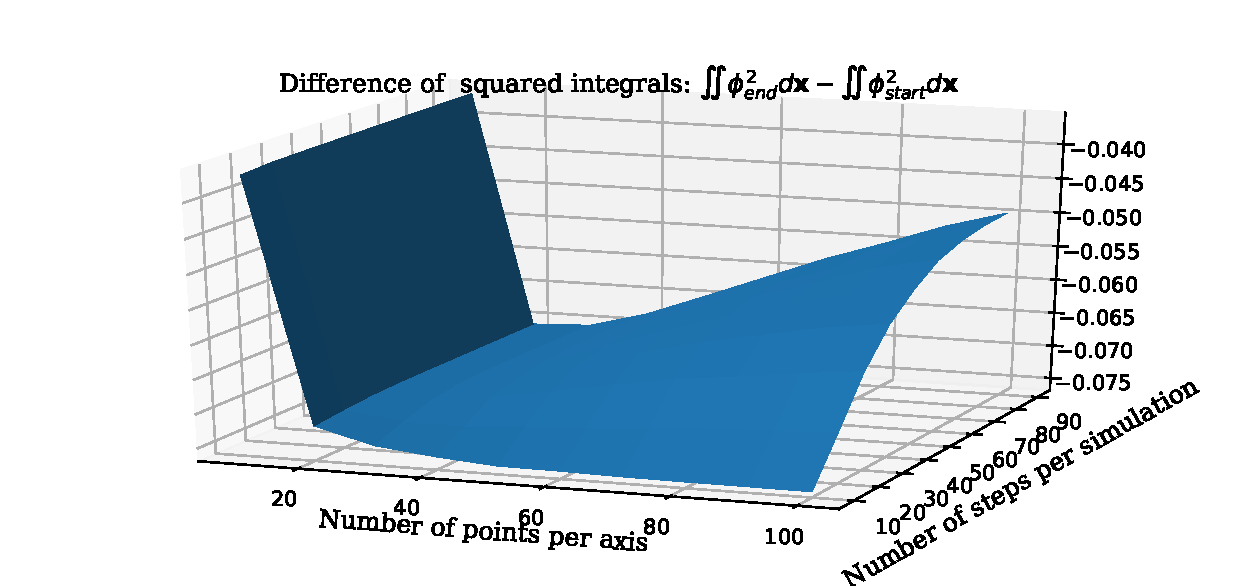
\includegraphics[width=\linewidth]{semi_lagrange_ex1.pdf}
	\caption{$ \Delta \phi^2 $ for a range of different number of iterations and number of grid points. Note $ \Delta t \propto N_t, \Delta_x \propto N_x $.}
	\label{fig:semi_lagrange_error}
\end{figure}
Notice the sign on the $ z $-axis. The difference does decrease as $ \Delta t $ and $ \Delta x $ are decreased, but seems to taper off towards some value. There is of course the sharp decrease in error when $ N_x = 10 $, but this is a pathological case, because $ \Delta x = 2$, and I am calculating the error for a Gaussian profile with $ \sigma_x=\sigma_y = 1 $. There simply is not enough points to sample the function accurately.

Lastly we view the evolution of the system with time, seen in figure \ref{fig:semi_traj}. And indeed, the scalar field rotates.

\begin{figure}
	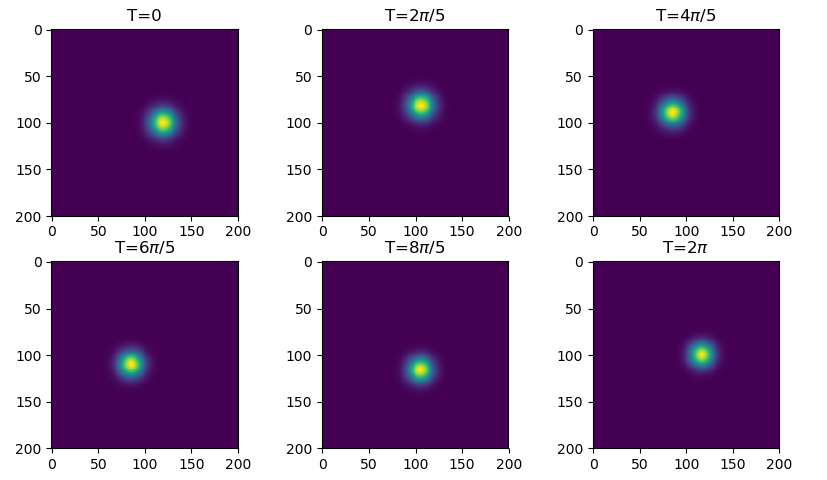
\includegraphics[width=\linewidth]{semi_lagrange_traj.png}
	\caption{Evolution of a Gaussian profile for $ \V{u}=(y, -x)^T $, with $ \Delta t = \pi/50 $. Shown after $ n $ iterations, with $ n\in \{0, 20, 40, 60, 80, 100\} $.}
	\label{fig:semi_traj}
\end{figure}

\section{Mean curvature flow with finite difference methods}
Next we turn our attention to solving the mean curvature flow equation for some signed distance field. Mean curvature flow is analogous to wrapping a tight string around an isosurface of a scalar field and then tightening the string such that it follows the isosurface at a higher value. The equation is given by
\begin{equation}\label{key}
	\diff{\phi}{t} = \nabla \D \frac{\nabla \phi}{||\grad \phi ||} = \kappa
\end{equation}
The right hand side of the equation can be rewritten as
\begin{equation}\label{key}
	\kappa = \frac{\grad \phi^T \grad \phi \tr H  - \grad\phi^T H \grad\phi}{||\grad\phi||^3}
\end{equation}
with $ H $ being the Hessian matrix.

\subsection{Signed Distance Fields}
A signed distance field is a scalar field describing the signed euclidian distance from each pixel of a black and white, binary image, to the nearest border between black and white, in units of pixels. The sign is such that white pixels are counted as inside, with a negative distance to the border. A one dimensional is seen in figure \ref{fig:signed_dist}, where the inside is defined to be $ x \in [5, 11] $. For points sufficiently close to a border will have a gradient of approximately 1.
\begin{figure}
	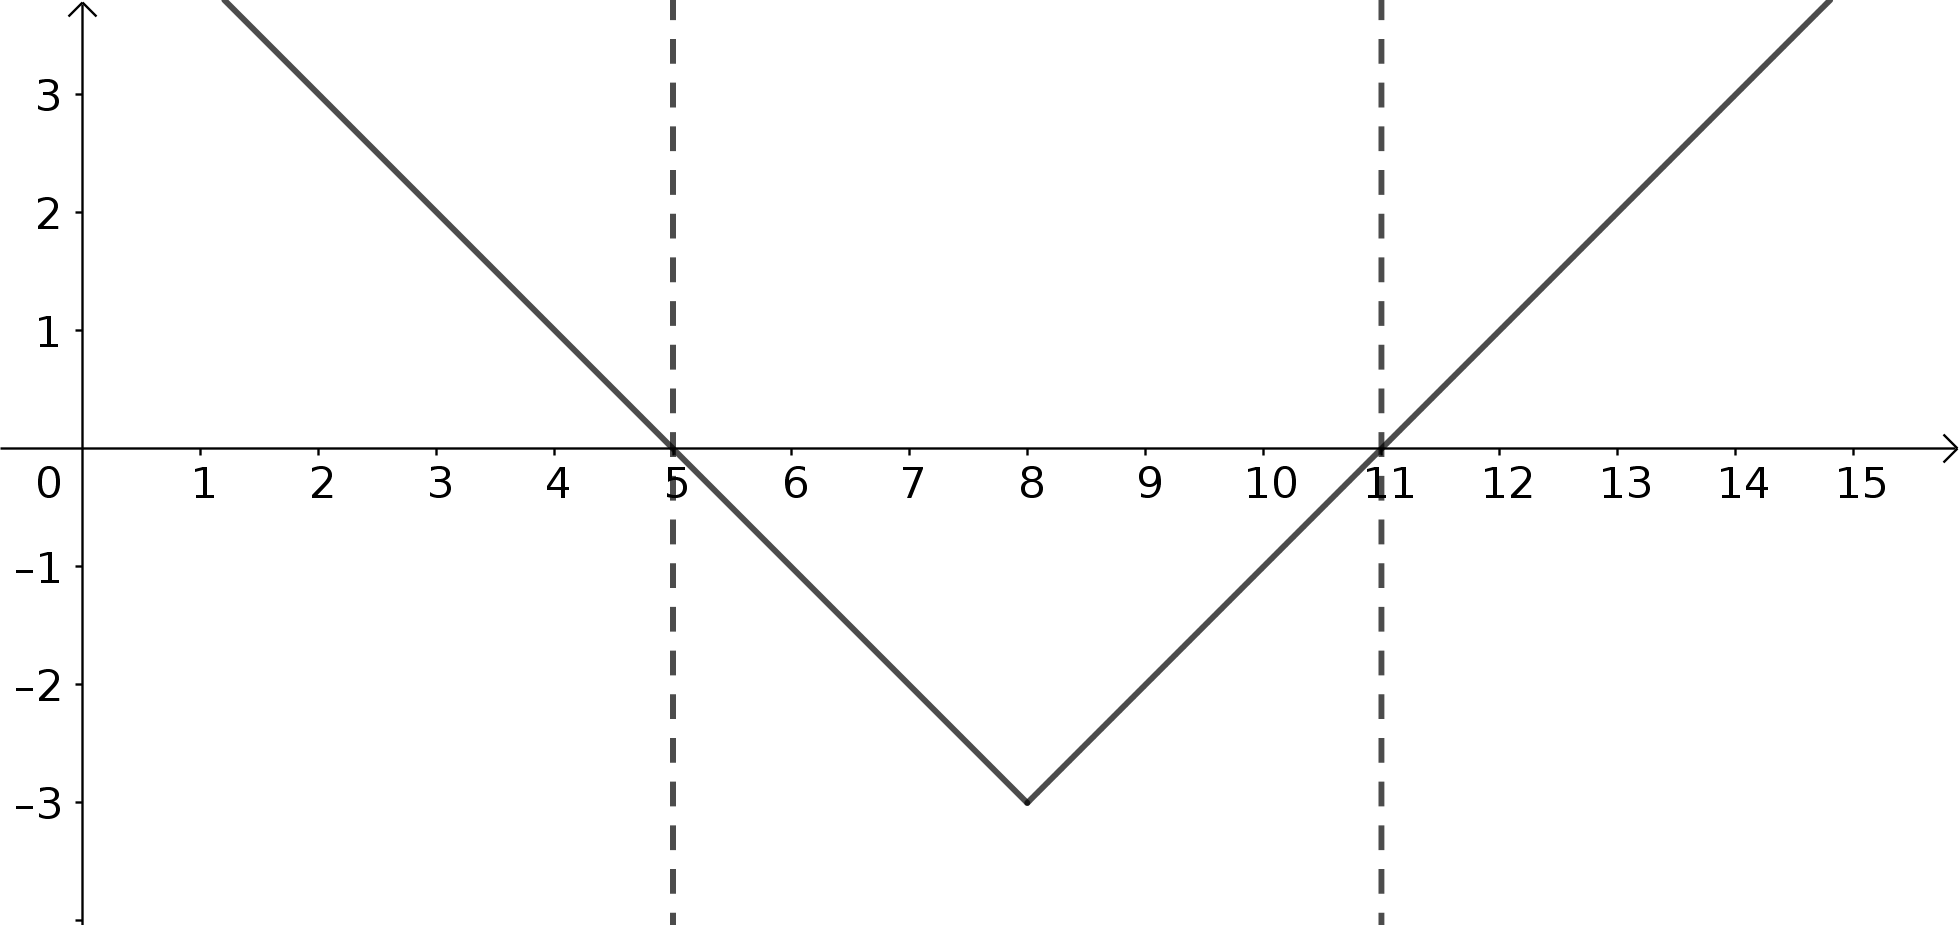
\includegraphics[width=\linewidth]{signed_distance_1d}
	\caption{A signed distance field in one dimension, with the inside as $ x \in [5, 11] $.}
	\label{fig:signed_dist}
\end{figure}


\subsection{Discretisation}
For the domain we employ a central difference approximation for each of the different spatial derivatives. This gives
\begin{equation}\label{key}
	\kappa \approx k = \frac{(D_x \phi)^2 D_{yy}\phi + (D_y \phi)^2 D_{xx}\phi - 2D_{xy}\phi D_x \phi D_y \phi}{\bb{(D_x\phi)^2 + (D_y\phi)^2}^{3/2}}
\end{equation}
where $ D $  is the central difference approximation, where the subscripts denote which variables are differentiated with respect to. For example the central difference approximation for the second order derivative with respect to $ x $:
\begin{equation}\label{key}
	D_{xx} \phi_{ij} = \frac{\phi_{i+1, j} - 2\phi_{i,j} + \phi_{i-1,j}}{\Delta x^2}.
\end{equation}
Some problems with this equation would be at or around points where the norm of the gradient disappears. This would result in possible division by zero, or just a very large value of $ k $.

A conservative maximum bound for the mean curvature is given by the inverse of the grid spacing: $ k_{\max} = \max(\Delta x, \Delta y)\inverse $. To remedy values that are too large one can clamp the value of $ k $ to between $ \pm k_{\max} $ by
\begin{equation}\label{key}
	k\leftarrow \max(-k_{\max}, \min(k, k_{\max})).
\end{equation}

For the temporal derivative we employ a first order forward difference to integrate in time:
\begin{equation}\label{key}
	\phi_{ij}^{t+\Delta t} = \phi_{ij}^t + \Delta t k_{ij}, 
\end{equation}
for some small $ \Delta t $.

This numerical scheme is conditionally stable, since too large a time step will lead to numerical blow up of the solution. The condition is called the CFL condition, and is given by
\begin{equation}\label{key}
	\Delta t \leq \frac{h}{2k_{\max}}, \quad h = \min(\Delta x, \Delta y)
\end{equation}
In our case, $ \Delta x = \Delta y = 1 $, and $ \Delta t \leq 1/2 $.

\subsection{Boundary conditions}
For a signed distance field, the boundary nodes will not have a fixed value, and as such a von Neumann boundary condition is preferable to a Dirichlet boundary condition. In general, the signed distance field will have a gradient of $ \pm 1 $ in each direction, so long as the node is sufficiently far away from the midpoint of a region. Since midpoints cannot occur at the boundary, it makes sense to extend the derivative to the boundary. For the left boundary this would mean $ d\phi_{1,j}/dx = d\phi{2_j}/dx$. This is implemented using ghost nodes and a central difference approximation:
\begin{equation}\label{key}
	\diff{\phi_{1,j}}{x} = \diff{\phi_{2,j}}{x} \quad \Rightarrow \quad \frac{\phi_{2,j} - \phi_{0,j}}{2\Delta x} = \frac{\phi_{3,j} - \phi_{1,j}}{2 \Delta x}
\end{equation}
Giving the updating formula for ghost nodes on the left boundary:
\begin{equation}\label{key}
	\phi_{0,j} = \phi_{1,j} + \phi_{2,j} - \phi_{3,j}.
\end{equation}

\subsection{Experiments}
The mean curvature flow equation should conserve the signed distance field properties. To test this I convert $ \phi $ back to a black and white image after the simulation using the mapping
\begin{equation}\label{key}
	\text{BW} = \begin{cases}
	1 & \phi < 0 \\
	0 & \phi \geq 0
	\end{cases}
\end{equation}
This mapping erases all information from $ \phi $, other than which parts of the field were inside and outside. Then I use the \texttt{bw2phi} function supplied by Kenny to generate the signed distance field from this new black and white image, introducing information to the system again. To quantify the error I calculate the RMS of the residual between the two images over the domain:
\begin{equation}\label{key}
	\text{Res} = \sum_{j=0}^N \sum_{i=1}^{N} (\phi_{\text{end}} - \phi_{\text{reconstructed}})^2 / N^2
\end{equation} 
This measurement should yield 0 if the simulation is a faithful representation of the mean curvature flow equation. This is tested on the sample image supplied by Kenny, resembling a flipped U, for a range of time step sizes (while keeping the ``absolute time'' unchanged, such that the end images should be equal across simulations). We of course expect the residual to trend towards zero as the time step is decreased. The results are shown in figure \ref{fig:residual}.

\begin{figure}
	\centering
	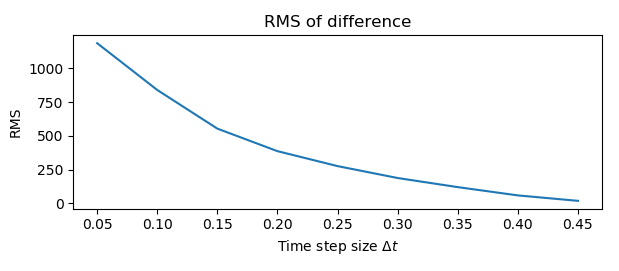
\includegraphics[width=\linewidth]{mean_curvature_flow_ex1.png}
	\caption{RMS between $  \phi_{\text{end}} $ and $ \phi_{\text{reconstructed}} $ as a function of $ \Delta t $, with $ T=500 $.}
	\label{fig:residual}
\end{figure}
\begin{figure}
	\centering
	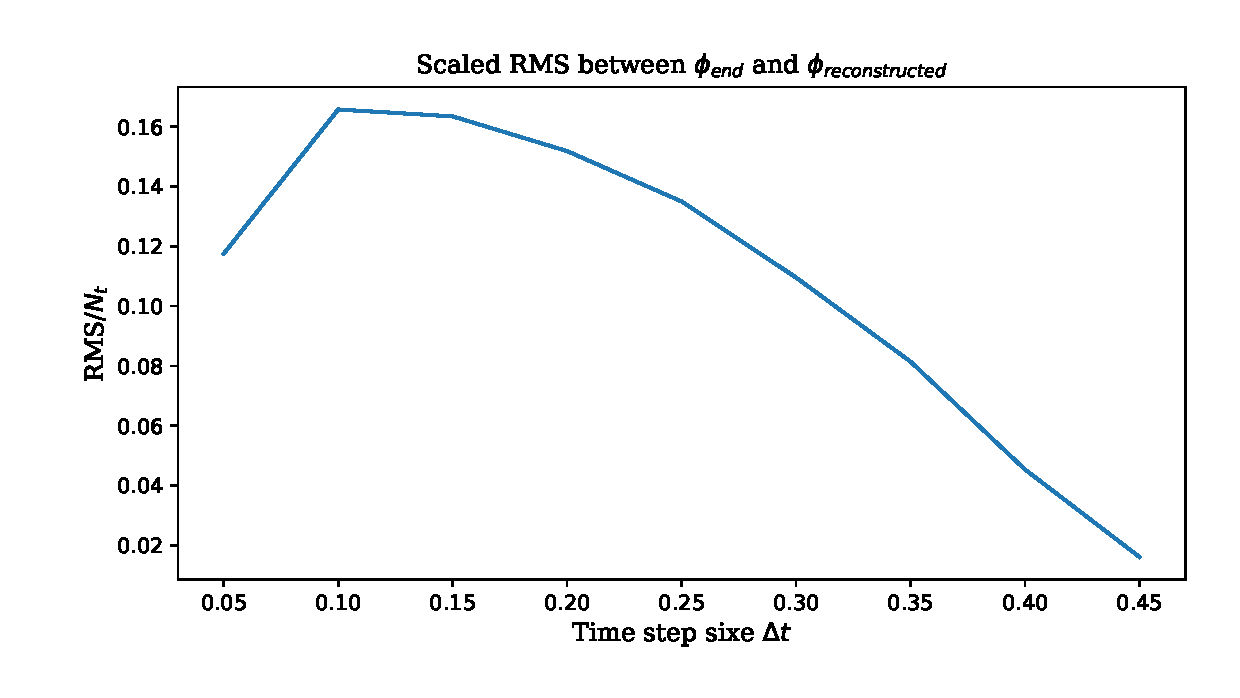
\includegraphics[width=\linewidth]{mean_curvature_flow_ex2.pdf}
	\caption{RMS between $  \phi_{\text{end}} $ and $ \phi_{\text{reconstructed}} $ as a function of $ \Delta t $. Scaled by the number of iterations: $ N_t = T/\Delta t $, for $ T=500 $.}
	\label{fig:scaled_residual}
\end{figure}
As seen in the figure, the residual actually increases as $ \Delta t $ is decreased, contrary to the expectation. This could however be a result of the number of iterations performed. For $ \Delta t = 0.45 $ a total of 1112 iterations were completed, while for $ \Delta t = 0.05 $ 10000 iterations were completed. Since more iterations equals more calculations, each of which includes truncation errors, it is natural to expect a higher residual as more iterations are performed. If we then also scale the residual by the number of iterations we get the error dependence on $ \Delta t $, per iteration. This is seen in figure \ref{fig:scaled_residual}.

The error still increases as $ \Delta t $ decreases, until some critical value of $ \Delta t \approx 0.1$ is reached. I would have liked to investigate this further, if time permitted.



Lastly, in figure \ref{fig:mcf_evol}, the signed distance field can be seen at a variety of times, with $ \Delta t=0.25 $, showing the time evolution of $ \phi $. As expected we see the contour of $ \phi=0 $ rounding at the corners and shrinking.
\begin{figure*}
	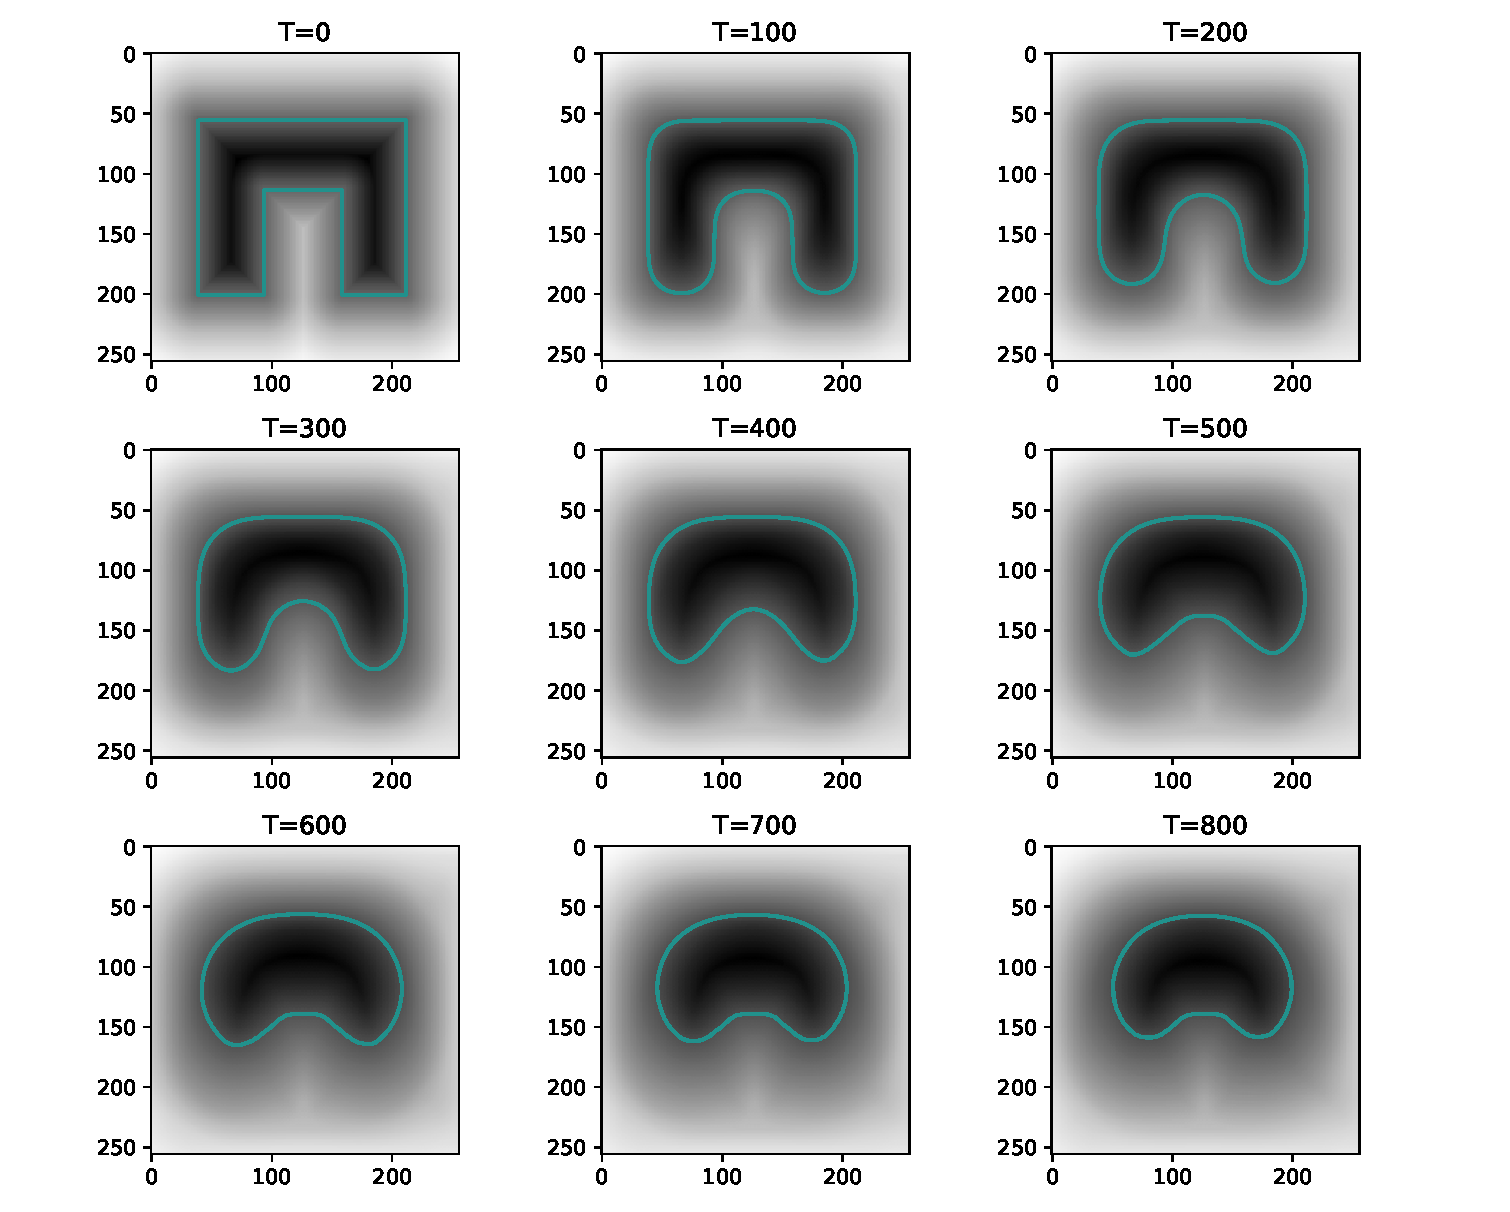
\includegraphics[width=\linewidth]{mean_curvature_evol.pdf}
	\caption{Evolution of the signed distance field generated from the sample image. $ \Delta t = 0.25 $.}
	\label{fig:mcf_evol}
\end{figure*}
\end{document}
